\documentclass[11pt]{article}

% Language setting
\usepackage[turkish]{babel}
\usepackage{pythonhighlight}

\usepackage[a4paper,top=2cm,bottom=2cm,left=2cm,right=2cm,marginparwidth=2cm]{geometry}

% Useful packages
\usepackage{amsmath}
\usepackage{graphicx}
\usepackage[colorlinks=true, allcolors=blue]{hyperref}
\usepackage{verbatim}
\usepackage{fancyhdr} % for header and footer
\usepackage{titlesec}
\usepackage{parskip}
\usepackage{hyperref}

\setlength{\parindent}{0pt}
\PassOptionsToPackage{hyphens}{url}\usepackage{hyperref}

\titleformat{\subsection}[runin]{\bfseries}{\thesubsection}{1em}{}

\pagestyle{fancy} % activate the custom header/footer

% define the header/footer contents
\lhead{\small{23BLM-4014 Yapay Sinir Ağları Ara Sınav Soru ve Cevap Kağıdı}}
\rhead{\small{Dr. Ulya Bayram}}
\lfoot{}
\rfoot{}

% remove header/footer on first page
\fancypagestyle{firstpage}{
  \lhead{}
  \rhead{}
  \lfoot{}
  \rfoot{\thepage}
}
 

\title{Çanakkale Onsekiz Mart Üniversitesi, Mühendislik Fakültesi, Bilgisayar Mühendisliği Akademik Dönem 2022-2023\\
Ders: BLM-4014 Yapay Sinir Ağları/Bahar Dönemi\\ 
ARA SINAV SORU VE CEVAP KAĞIDI\\
Dersi Veren Öğretim Elemanı: Dr. Öğretim Üyesi Ulya Bayram}
\author{%
\begin{minipage}{\textwidth}
\raggedright
Öğrenci Adı Soyadı: İlkay Biçici\\ % Adınızı soyadınızı ve öğrenci numaranızı noktaların yerine yazın
Öğrenci No: 180401002
\end{minipage}%
}

\date{14 Nisan 2023}

\begin{document}
\maketitle

\vspace{-.5in}
\section*{Açıklamalar:}
\begin{itemize}
    \item Vizeyi çözüp, üzerinde aynı sorular, sizin cevaplar ve sonuçlar olan versiyonunu bu formatta PDF olarak, Teams üzerinden açtığım assignment kısmına yüklemeniz gerekiyor. Bu bahsi geçen PDF'i oluşturmak için LaTeX kullandıysanız, tex dosyasının da yer aldığı Github linkini de ödevin en başına (aşağı url olarak) eklerseniz bonus 5 Puan! (Tavsiye: Overleaf)
    \item Çözümlerde ya da çözümlerin kontrolünü yapmada internetten faydalanmak, ChatGPT gibi servisleri kullanmak serbest. Fakat, herkesin çözümü kendi emeğinden oluşmak zorunda. Çözümlerinizi, cevaplarınızı aşağıda belirttiğim tarih ve saate kadar kimseyle paylaşmayınız. 
    \item Kopyayı önlemek için Github repository'lerinizin hiçbirini \textbf{14 Nisan 2023, saat 15:00'a kadar halka açık (public) yapmayınız!} (Assignment son yükleme saati 13:00 ama internet bağlantısı sorunları olabilir diye en fazla ekstra 2 saat daha vaktiniz var. \textbf{Fakat 13:00 - 15:00 arası yüklemelerden -5 puan!}
    \item Ek puan almak için sağlayacağınız tüm Github repository'lerini \textbf{en geç 15 Nisan 2023 15:00'da halka açık (public) yapmış olun linklerden puan alabilmek için!}
    \item \textbf{14 Nisan 2023, saat 15:00'dan sonra gönderilen vizeler değerlendirilmeye alınmayacak, vize notu olarak 0 (sıfır) verilecektir!} Son anda internet bağlantısı gibi sebeplerden sıfır almayı önlemek için assignment kısmından ara ara çözümlerinizi yükleyebilirsiniz yedekleme için. Verilen son tarih/saatte (14 Nisan 2023, saat 15:00) sistemdeki en son yüklü PDF geçerli olacak.
    \item Çözümlerin ve kodların size ait ve özgün olup olmadığını kontrol eden bir algoritma kullanılacaktır. Kopya çektiği belirlenen vizeler otomatikman 0 (sıfır) alacaktır. Bu nedenle çözümlerinizi ve kodlarınızı yukarıda sağladığım gün ve saatlere kadar kimseyle paylaşmayınız.
    \item Bu vizeden alınabilecek en yüksek not 100'dür. Toplam aldığınız puan 100'ü geçerse, aldığınız not 100'e sabitlenecektir.
    \item LaTeX kullanarak PDF oluşturanlar öz geçmişlerine LaTeX bildiklerini de eklemeyi unutmasınlar :)
    \item Bu vizedeki soruların çözümleri ve tex dosyası için istediğiniz kadar sayıda Github repository'si oluşturabilirsiniz. Sadece yukarıda belirttiğim tarihlerde (14 Nisan 2023 saat 15:00 ile 15 Nisan 2023 saat 15:00 arasında) public yapmayı/halka açmayı ve Github profilinizi de öz geçmişinize eklemeyi unutmayın :)
    \item Bilgisayarınıza hiçbir program kurmadan, Overleaf, Google Colab, Kaggle gibi ortamlar üzerinden bu vizeyi tamamlamanız mümkün. İyi çalışmalar!!
\end{itemize}

(Ekstra 5 puan) \href{https://github.com/ilkay-bicici/yapaysiniraglariornekler.git}{Odevin GitHub Linki}

\newpage
\section{(Toplam 10 Puan) Hopfield Networks:}

\subsection{(2 Puan)} \textbf{ChatGPT’ye size Hopfield Network’ler ile ilgili detaylı bilgi vermesini isteyin. Sorduğunuz soruyu, ChatGPT'nin çıkartığı cevabı aşağı koyun. Bu cevapta anlamadığınız terimleri de ChatGPT’ye sorup, sorduğunuz soruları ve ChatGPT’nin verdiği cevapları da sırayla aşağı koyun.}


BEN: bana hopfield networkler ile ilgili detaylı bilgi ver.

CHAT GPT: Hopfield ağları, bellek modelleri olarak kullanılan yapay sinir ağlarıdır. Bu ağlar, bağlantılı bir matris kullanarak basit bir şekilde tasarlanmıştır ve bir hafıza kapasitesi sağlamak için kullanılırlar.

Hopfield ağları, asenkron ve senkron çalışma modlarına sahiptir. Asenkron modda, her bir düğüm (nöron) zaman içinde sırayla güncellenir, yani sadece bir düğüm değiştirilir. Senkron modda ise, tüm düğümler aynı anda güncellenir.

Ağın hafıza kapasitesi, öğelerin doğru bir şekilde tanınması için gereken girdi vektörlerinin sayısı ile sınırlıdır. Hopfield ağı, bir girdi vektörü aldığında, bu vektörü bellek matrisinde en yakın benzerliğe sahip olan öğeyle eşleştirmeye çalışır. Aynı zamanda, ağ gürültüye dayanıklıdır ve girdi vektörlerindeki hataları düzeltebilir.

Hopfield ağları, özellikle optimizasyon problemleri için kullanışlıdır. Optimizasyon problemleri, bir dizi kısıtlama altında, bir hedef fonksiyonun minimum veya maksimum değerini bulmakla ilgilidir. Hopfield ağı, bu tür problemleri çözmek için enerji fonksiyonu olarak adlandırılan bir objektif fonksiyon kullanır.

Ağ, birbirine bağlı nöronlardan oluşur ve nöronlar arasındaki bağlantılar, bellek matrisindeki her öğe için bir ağırlık matrisiyle belirlenir. Hopfield ağı, simetrik bir ağırlık matrisi kullanır, bu da belleğin kararlılığı için gereklidir. Ayrıca, ağın çıktısı, bir adım fonksiyonu kullanılarak belirlenir.

Hopfield ağları, özellikle sınırlı bellekli sistemler için kullanışlıdır. Bu ağlar, birçok farklı alanda kullanılmaktadır, örneğin veri sıkıştırma, veri kodlama, veri analizi, veri işleme ve modelleme gibi konularda faydalıdır.

BEN: hopfield networkte bellek matrisi nedir?

CHAT GPT: Hopfield ağı, bir bellek matrisi kullanarak bir hafıza kapasitesi sağlar. Bellek matrisi, ağın öğrenmesini ve sonrasında tanıma yapmasını sağlayan öğelerin depolandığı bir matristir.

Bellek matrisi, ağın yapısı ve işlevi için çok önemlidir. Bu matris, ağın hafıza kapasitesini belirler ve ağın bir girdi vektörü aldığında bellek matrisinde en yakın benzerliğe sahip olan öğeyle eşleştirmesine olanak tanır.

Bellek matrisi, ağın her bir öğesinin boyutu ile belirlenir. Her bir öğe, genellikle 0 veya 1 gibi ikili bir değerle ifade edilir. Bellek matrisindeki öğeler, ağın simetrik bir ağırlık matrisi kullanarak bağlantılı nöronları arasındaki bağlantıları belirleyen bir öğrenme süreciyle oluşturulur.

Ağ, bir girdi vektörü aldığında, bu vektörü bellek matrisindeki en yakın benzerlikle eşleştirmeye çalışır. Bu işlem, ağın gürültüye dayanıklı olmasını ve girdi vektörlerindeki hataları düzeltmesini sağlar.

Hopfield ağları, bellek matrisindeki öğelerin sayısı ile sınırlı bir hafıza kapasitesine sahiptir. Bu nedenle, bellek matrisi boyutu, ağın performansını ve bellek kapasitesini etkileyen önemli bir faktördür.

BEN: hopfield ağlarında kullanılan enerji fonksiyonu hakkında bilgi ver

CHAT GPT: Hopfield ağları, enerji fonksiyonu olarak adlandırılan bir objektif fonksiyon kullanırlar. Bu fonksiyon, ağın öğrenme ve tanıma işlemlerinde kullanılır.

Enerji fonksiyonu, ağın her bir öğesinin bellek matrisindeki değerleri ile bağlantılı nöronlar arasındaki ağırlıkları kullanarak hesaplanır. Bu fonksiyon, bir öğenin diğer öğelerle olan ilişkisini gösterir ve ağın hafıza kapasitesini belirler.

Enerji fonksiyonu, bir öğenin bellek matrisindeki değerleri ve bağlantılı nöronlar arasındaki ağırlıkların çarpımının toplamını hesaplayan bir matematiksel ifade şeklindedir. Bu toplam, ağın enerji seviyesini temsil eder.

Ağın amacı, enerji fonksiyonunun minimum seviyesine ulaşmaktır. Minimum seviyeye ulaşmak, bellek matrisindeki girdi vektörüne en yakın benzerlikteki öğeyi belirlemek anlamına gelir.
Ağın öğrenme işlemi, enerji fonksiyonunun minimum değerine ulaşması için ağırlık matrisindeki değerleri güncellemek şeklinde gerçekleşir. Bu güncelleme işlemi, bir öğenin değerini değiştirdiğinde, diğer öğelerin de değerlerinde bir değişiklik meydana gelir.

Hopfield ağlarının enerji fonksiyonu, özellikle optimizasyon problemleri için kullanışlıdır. Bu fonksiyon, ağın en uygun çözümü bulmasına yardımcı olur ve özellikle sınırlı bellekli sistemler için çok etkilidir.

BEN: objektif fonksiyon nedir ?

CHAT GPT: Objektif fonksiyon, matematiksel bir ifade olarak belirtilen ve genellikle optimizasyon problemlerinde kullanılan bir fonksiyondur. Bir problemdeki hedefi veya amaçları ifade eden bir fonksiyondur.

Optimizasyon problemleri, belirli bir amaç fonksiyonunu en iyi hale getirmek için değişkenlerin değerlerini ayarlamakla ilgilidir. Bu amaç fonksiyonu, objektif fonksiyon olarak adlandırılır.

Objektif fonksiyon, belirli bir işlemin başarısını ölçmek için kullanılan bir ölçüttür. Örneğin, bir öğrenme algoritması tarafından optimize edilen ağırlıkların performansını ölçmek için bir hata fonksiyonu olarak kullanılabilir.

Objektif fonksiyonlar, minimum veya maksimum değeri en aza indirmek veya en yüksek değeri elde etmek için optimize edilirler. Örneğin, bir regresyon modelinde, objektif fonksiyon, gerçek ve tahmini değerler arasındaki farkı en aza indirmek için optimize edilir.

Birçok alanda kullanılan objektif fonksiyonlarının örnekleri arasında maliyet fonksiyonları, kayıp fonksiyonları, performans ölçütleri ve doğruluk ölçütleri gibi birçok çeşit bulunmaktadır.

BEN: hopfield ağlarında tüm nöronlar birbirlerine bağlı mıdır ?

CHAT GPT: Evet, Hopfield ağlarında tüm nöronlar birbirlerine bağlıdır. Hopfield ağı, tam bağlı bir yapay sinir ağı modelidir, yani her nöron, ağdaki her diğer nöronla bağlantılıdır. Bu bağlantılar, ağı oluşturan tüm nöronların bellek işlevini yerine getirmesini sağlar. 

Bu bağlantılar, ağırlık matrisi olarak adlandırılan bir matris ile temsil edilir ve matrisin her elemanı, iki nöron arasındaki bağlantı ağırlığını belirtir.

BEN: peki hopfield networkün normal nöral networkten farkı nedir ?

CHAT GPT: Hopfield ağı, normal yapay sinir ağı modellerinden farklıdır çünkü sadece bellek işlevi için kullanılır. Normal sinir ağları, bir girdi vektörünü alır ve bir çıktı vektörü üretmek için eğitilirken, Hopfield ağları, bir bellek matrisini depolayabilen ve daha sonra bu matristeki verileri hatırlayabilen bir modeldir. Bu nedenle, Hopfield ağı, sınırlı bellekli sistemler için özellikle yararlıdır.

Hopfield ağı, ayrıca geri yayılım algoritması gibi bir öğrenme algoritmasına ihtiyaç duymaz. Bunun yerine, ağın öğrenmesi enerji fonksiyonu adı verilen bir matematiksel fonksiyon kullanılarak gerçekleştirilir. Bu enerji fonksiyonu, ağın hafıza kapasitesini belirler ve ağın amacı, enerji fonksiyonunun minimum seviyesine ulaşmaktır.

Hopfield ağları, normal sinir ağlarından daha az esnek olabilirler ve verilerin sadece önceden belirlenmiş bellek matrislerinde saklanabildiği için, yeni verilerin eklenmesi daha zor olabilir. Ancak, optimizasyon problemleri için yararlıdırlar ve özellikle dar bellekli sistemler için kullanışlıdırlar.

BEN: hopfield ağlarının gürültüye dayanıklı olması ne demek ?
CHAT GPT: Hopfield ağlarının gürültüye dayanıklı olması, bellek matrisindeki verilerdeki bazı hatalar veya eksikliklerle bile hatırlama işlemini başarabilme yeteneğine sahip olması anlamına gelir.

Hopfield ağı, bir bellek matrisindeki verileri hatırlama amacıyla kullanılır. Bu bellek matrisi, ağın öğrenme sürecinde ağırlıkların ayarlandığı ve daha sonra hatırlama için kullanıldığı bir dizi öğeden oluşur. Hopfield ağları, bellek matrisindeki verilerin bir kısmı kaybedilse bile, geri kalan verileri doğru bir şekilde hatırlayabilir.

Bu, özellikle gerçek dünya uygulamalarında önemlidir çünkü verilerdeki gürültü veya hatalar her zaman olasıdır. Örneğin, bir resim tanıma uygulamasında, resimdeki bir parça eksik veya yanlış olabilir, ancak Hopfield ağı, eksik veya yanlış bilgiyle bile, resmin tamamını doğru bir şekilde tanımlayabilir. Bu nedenle, Hopfield ağları, gürültüye karşı dayanıklılık gerektiren uygulamalarda kullanışlıdır.

BEN: hopfield ağlarının çeşitleri var mıdır ? varsa bunlar nelerdir?

CHAT GPT:

1-Discrete Hopfield Network: Bu ağ, sadece iki durum (0 veya 1) ile ifade edilen kategorik verileri işlemek için tasarlanmıştır. Bellek matrisindeki her öğe, ağırlıkların ayarlandığı ve daha sonra hatırlama için kullanıldığı bir dizi bit değeridir.

2-Continuous Hopfield Network: Bu ağ, sürekli verileri işlemek için tasarlanmıştır. Bellek matrisindeki her öğe, gerçel sayılarla ifade edilen bir dizi değerdir.

3-Asymmetric Hopfield Network: Bu ağ, asimetrik ağırlıklar kullanarak tasarlanmıştır. Bu ağ, her bir ağ öğesinin bellek matrisinde farklı bir ağırlığa sahip olabileceği anlamına gelir. Bu ağ, simetrik ağırlıkların kullanılamadığı durumlarda kullanışlıdır.

4-Structured Hopfield Network: Bu ağ, veriler arasındaki özel ilişkileri dikkate alarak tasarlanmıştır. Bu nedenle, bellek matrisindeki veriler arasındaki ilişkileri belirlemek için farklı yöntemler kullanılır.

5-Bidirectional Associative Memory (BAM): Bu ağ, iki bellek matrisi arasındaki ilişkileri öğrenir ve bu matrislerdeki verileri birbirleriyle ilişkilendirir. BAM, simetrik ağırlıklar kullanır ve hem geri hatırlama hem de ileri hatırlama işlemleri yapabilir.

Bu farklı türdeki Hopfield ağları, farklı veri tipleri ve ilişkileri için kullanışlıdır.

BEN: Hopfield ağı, bir girdi vektörü aldığında, bu vektörü bellek matrisinde en yakın benzerliğe sahip olan öğeyle eşleştirmeye çalışır. Bu yüzden mi hopfield ağları gürültüye dayanıklıdır ?

CHAT GPT: Evet, doğru. Hopfield ağları, bellek matrisindeki öğeler arasındaki benzerlikleri öğrendikleri için girdi vektörünü bellek matrisindeki en yakın benzerlikle ilişkilendirmeye çalışırlar. Bu, gürültüye dayanıklı olmalarına yardımcı olur çünkü bellek matrisindeki bir öğeye benzerlik göstermeyen gürültülü bir girdi vektörü, ağın en yakın benzerlikle eşleştirme işlemi sırasında bir hata yapmasına neden olur.

Ancak, Hopfield ağları sadece bir düzeyde gürültüye dayanıklıdır. Yani, bellek matrisindeki öğeler arasındaki benzerlik farkı çok küçük ise, Hopfield ağı hatırlama işlemi sırasında hatalar yapabilir.

BEN: hopfield ağlarında adım fonksiyonu nedir ?

CHAT GPT: Hopfield ağlarında adım fonksiyonu, ağın çıkışını hesaplamak için kullanılan bir aktivasyon fonksiyonudur. Adım fonksiyonu, bir eşik değeri üzerindeki girdileri 1'e, eşik değerinin altındaki girdileri ise 0'a eşitler. Matematiksel olarak, eşik değeri theta olan bir adım fonksiyonu f(x), şu şekilde tanımlanır:

$f(x) = \frac{f(x) = 1, x ≥ theta}

$f(x) = \frac{f(x) = 0, x < theta}

Hopfield ağlarında, her nöronun çıkışı adım fonksiyonu ile hesaplanır. Bu çıkış değerleri, ağın diğer nöronlarına girdi olarak iletilir ve ağın toplam enerjisi hesaplanır. Enerji fonksiyonunun minimize edilmesi için iteratif bir süreç kullanılarak ağın çıkışı güncellenir. Bu süreç, Hopfield ağının hatırlama işlemini gerçekleştirir.

BEN: Hopfield ağının hatırlama işlemi ile öğrenme işlemi arasında bir fark var mıdır ? varsa bu fark veya farklar nelerdir ?

CHAT GPT: Evet, Hopfield ağının hatırlama işlemi ile öğrenme işlemi arasında farklar vardır.

Öğrenme işlemi, Hopfield ağının bellek matrisinde saklanacak olan örneklerin öğrenilmesini içerir. Bu işlem, bellek matrisindeki örneklerin arasındaki benzerlikleri hesaplar ve ağı bu örnekleri hatırlamak için ayarlar. Bu işlem, ağın sinir ağırlıklarını ayarlayarak gerçekleştirilir ve sadece bir kez yapılır.

Hatırlama işlemi, ağa sunulan bir girdi vektörünü bellek matrisindeki en yakın örnek ile eşleştirmeyi amaçlar. Bu işlem, ağın önceden öğrendiği örnekler arasında benzerlik ölçerek gerçekleştirilir. Hatırlama işlemi, ağın sinir ağırlıklarını değiştirmez ve birden fazla kez yapılabilir.

Bu nedenle, öğrenme işlemi ağın ilk kurulumunu ve bellek matrisine örneklerin öğrenilmesini içerirken, hatırlama işlemi öğrenilen örneklerin hatırlanmasını içerir ve ağın herhangi bir zaman diliminde birden fazla kez yapılabilir.


\subsection{(8 Puan)} \textbf{ChatGPT’nin açıklamalarından ne anladığınızı buraya kendi kelimelerinizle özetleyin. Örneğin ``Hopfield Network nedir? Ne işe yarar? Neden bilmemiz gerekir bunu? Gerçek hayatta kullanılıyor mu?'' gibi. Anlamadığınız kısımlar varsa ve ChatGPT’nin açıklamaları yeterli gelmezse internet dahil farklı kaynaklardan araştırıp, bilgilerin doğruluğunu sorgulamakta serbestsiniz. Konuyu doğru anlayıp anlamamanız puana etki edecektir. Kullandığınız kaynakları da belirtin!}

Hopfield Network bir çeşit yapay sinir ağıdır. Bu ağ modelinde tüm nöronlar birbirine bağlıdır. Bu bağlantılar sayesinde bellek işlevine sahiptir. Nöronların bağlantıları için simetrik (devriği kendisine eşit) ağırlık matrisi kullanılır. Hopfield Network'ün hafıza kapasitesini input vektörleri belirler. Yine hopfield networkte yer alan bellek matrisi de ağın permormansını etkiler.
Hopfield ağlarının  senkron ve asenkron çalışma modları vardır. Asenkron modda nöronlar zamanla güncellenirken senkron modda düğümlerin hepsi aynı anda güncellenir.

Hopfield  ağına bir vektör geldiğinde bu vektör, bellek matrisindeki mümkün olan en yakın örnek ile eşleştirilmeye çalışılır. Hatırlama işlemi bu şekilde gerçekleştirilir. Ayrıca bu sayede bozuk verilerin yeniden oluşturulmasında hopfield ağları kullanılır.  Bu duruma kısaca gürültüye dayanıklı olmasıdır. Ancak bellek matrisinde yer alan örnekler birbirine benziyorsa hopfield modeli hata yapabilir.

Hopfield ağlarında,  adım fonksiyonu adı verilen aktivasyon fonksiyonu, her nöronun çıkış değerini uygulanır ve bu değerler  diğer  nöronların girişine yönlendirilir.  Süreç devam ettikçe enerji fonksiyonu azaltılır. 

Hopfield  networkun öğrenmesi,  ağırlık matrisindeki değerlerinin güncellenmesi sonucu enerji fonksiyonunun minimum değerine ulaşmasıyla sağlanır.  Hatırlama işlemi de ağa verilen girdi vektörünün  bellek matrisindeki örnekler ile kıyaslanması şeklinde gerçekleşir.

Hopfield ağları,  sınırlı belleğe sahip olan sistemler için  elverişlidir. Ayrıca optimizasyon problemlerinde de kullanılırlar.  Örnekler verecek olursak:

Yüz tanıma sistemi, örüntü tanıma sistemi, hedef tanıma sistemleri, veri sıkıştırma, işleme, analiz etme ve ve modellemede kullanılır. Bu ağlar eksik veriler ile de çalışabildiklerinden gerçek hayat problemlerinde de kullanılırlar.

Ayrıca  hopfield network’ün discrete, continuous, asymmetric, structured, bidirectional associative memory gibi türleri bulunur.

KULLANDIĞIM DİĞER KAYNAKLAR:

\url{https://www.geeksforgeeks.org/hopfield-neural-network/}

\url{https://towardsdatascience.com/hopfield-networks-neural-memory-machines-4c94be821073}

\url{https://medium.com/@batincangurbuz/hopfield-a%C4%9F-modeli-hopfield-network-hn-ccf1548ca432}

\url{https://dna.caltech.edu/courses/cns187/problemsets/Hopfield_intro.pdf}


\section{(Toplam 10 Puan) Boltzman Machine:}

\subsection{(2 Puan)} \textbf{ChatGPT’ye size Boltzman Machine ilgili detaylı bilgi vermesini isteyin. Sorduğunuz soruyu, ChatGPT'nin çıkartığı cevabı aşağı koyun. Bu cevapta anlamadığınız terimleri de ChatGPT’ye sorup, sorduğunuz soruları ve ChatGPT’nin verdiği cevapları da sırayla aşağı koyun.}

BEN: Bana boltzman Machine ilgili detaylı bilgi ver.

CHATGPT: Boltzmann makineleri, istatistiksel mekanikte kullanılan ve makine öğrenmesinde de kullanılan bir tür yapay sinir ağıdır. İsmi, ünlü fizikçi Ludwig Boltzmann'ın adından gelmektedir.

Bir Boltzmann makinesi, veri setindeki örnekleri sınıflandırmak veya modellemek için kullanılır. Makine, girdi olarak verilen örnekleri alır ve bunları belirli bir sayıda gizli birimle ilişkilendirir. Bu gizli birimler, modelin girdileri nasıl işlediği hakkında bilgi sağlarlar. Daha sonra, makine, bu gizli birimlerin durumuna göre, örnekleri sınıflandırmak veya modellemek için kullanılan çıktıları üretir.

Boltzmann makineleri, diğer yapay sinir ağlarına göre daha esnek bir yapıya sahiptirler. Bu nedenle, özellikle belirsizliğin yüksek olduğu durumlarda, örneğin ses ve görüntü tanıma gibi, daha iyi sonuçlar verebilirler. Ancak, Boltzmann makinelerinin eğitimi diğer yapay sinir ağlarına göre daha zordur.

Boltzmann makineleri, özellikle sinirbilim, psikoloji ve bilişsel bilim gibi alanlarda da araştırma konusu olmuştur. Bu alanlarda, Boltzmann makinelerinin insan beyninin işleyişini anlamak için kullanılabileceği düşünülmektedir

BEN: istatiksel mekanik nedir ?

CHATGPT: İstatistiksel mekanik, fizikteki bir dal olarak, atomik veya moleküler düzeydeki sistemlerin davranışlarını istatistiksel yöntemler kullanarak modelleyen bir disiplindir. İstatistiksel mekanik, termodinamik prensiplerini mikroskobik düzeyde açıklamak için kullanılır.

İstatistiksel mekanik, bir sistemin içindeki parçacıkların hareketlerini, enerji dağılımını ve etkileşimlerini hesaplayarak, makroskopik özelliklerini tahmin eder. Örneğin, termodinamiksel özellikleri (sıcaklık, basınç, hacim, entropi vb.) hesaplamak için kullanılabilir.

İstatistiksel mekanik, fizik, kimya, mühendislik, malzeme bilimi ve biyofizik gibi birçok alanda kullanılır. Bu alanda çalışanlar, atomik ve moleküler düzeydeki sistemlerin davranışları hakkında daha detaylı bilgi edinmek için istatistiksel yöntemleri kullanır.

BEN: Boltzmann makinelerinde gizli birim nedir ?

CHATGPT: Bir Boltzmann makinesinde, girdilerin işlenmesi ve örüntülerin öğrenilmesi için kullanılan gizli birimler, modelin özelliğidir. Gizli birimler, modelin öğrenilmesi sırasında otomatik olarak belirlenir ve veri setindeki örnekler arasındaki özellikleri belirlemek için kullanılır.

Gizli birimler, girdi verilerinin işlendiği ve çıktıların hesaplandığı ağın "gizli" kısmını oluştururlar. Bu gizli kısım, verilerin özelliklerini daha derinlemesine öğrenmek için kullanılır ve veri setindeki ilişkileri daha iyi modellemeye yardımcı olur.

Bir Boltzmann makinesinde, her gizli birim, girdi verilerinden gelen bağlantılarla ve çıktı verilerine giden bağlantılarla bağlantılıdır. Gizli birimlerin aktivasyonları, bu bağlantıların ağırlıklarına bağlıdır ve ağın çıktısını belirlemek için kullanılır.

Gizli birimler, Boltzmann makinesinin öğrenme sürecinde önemli bir rol oynarlar ve doğru bir şekilde ayarlanmaları, modelin başarısı için önemlidir.

BEN: Boltzmann makinelerinin eğitimi diğer yapay sinir ağlarına göre neden daha zordur ?

CHATGPT: Boltzmann makineleri, diğer yapay sinir ağı modellerine göre eğitimi daha zor olan bir yapay sinir ağıdır. Bunun nedenleri şunlar olabilir:

1-Eğitim Algoritması: Boltzmann makinelerinin eğitimi, diğer yapay sinir ağı modellerine göre daha yavaş ve daha karmaşıktır. Eğitim algoritmaları, Markov Zinciri Monte Carlo (MCMC) gibi daha gelişmiş teknikleri içerir ve daha fazla hesaplama gücü gerektirir.

2-Büyük Veri Setleri: Boltzmann makineleri, büyük veri setleri üzerinde eğitildiğinde, öğrenme süreci oldukça yavaş olabilir. Bu nedenle, daha büyük örneklem büyüklüklerine ihtiyaç duyarlar.

3-Sınır Durumları: Boltzmann makineleri, bazı sınır durumlarına karşı hassas olabilir. Örneğin, veri setindeki sınıfların dengesiz dağılımı, modelin öğrenmesini zorlaştırabilir. Ayrıca, ağdaki birçok bağımsız parametre nedeniyle, ağın overfitting yapması da mümkündür.

4-Parametre Sayısı: Boltzmann makineleri, diğer yapay sinir ağı modellerine göre daha fazla parametreye sahiptir. Bu da, modelin eğitim sürecini daha karmaşık hale getirir ve daha fazla hesaplama gücü gerektirir.

Bu nedenlerden dolayı, Boltzmann makinelerinin eğitimi daha zor olsa da, veri setleri üzerindeki doğruluğu ve esnekliği, bazı durumlarda diğer yapay sinir ağı modellerinden daha iyi sonuçlar verir.

BEN: Boltzmann makineleri nasıl çalışır ?

CHATGPT: Bir Boltzmann makinesi, bir tür enerji tabanlı olasılık modelidir. Veri setinin özelliklerini öğrenmek için kullanılır ve girdi verilerini alırken, bu verileri işler ve bir çıktı üretir.

Bir Boltzmann makinesi, iki tip birimden oluşur: görünür birimler ve gizli birimler. Görünür birimler, veri setindeki gözlemlenen değişkenlere karşılık gelirken, gizli birimler, veri setindeki gözlemlenemeyen değişkenlere karşılık gelir.

Bir Boltzmann makinesi, tüm olası veri örneklerinin bir enerji değerini hesaplar. Daha sonra, veri örneklerinin olasılık dağılımını hesaplamak için bu enerji değerlerini kullanır.

Bir Boltzmann makinesinin işleyişi, görünür ve gizli birimlerin birbirleriyle etkileşimlerine dayanır. Bu etkileşimler, birimler arasındaki bağlantıların ağırlıkları tarafından belirlenir.

Bir Boltzmann makinesi, iki aşamalı bir işleme sahiptir: öncül ölçümler ve ters ölçümler. Öncül ölçümler, görünür birimlerin değerlerinin sabitlenmesi ve ardından gizli birimlerin değerlerinin rastgele seçilmesiyle gerçekleştirilir. Ters ölçümler, gizli birimlerin değerlerinin sabitlenmesi ve ardından görünür birimlerin değerlerinin rastgele seçilmesiyle gerçekleştirilir.

Bir Boltzmann makinesi, öncül ve ters ölçümlerin birçok tekrarı sonucu, veri setindeki örüntüleri öğrenir. Öğrenme işlemi, enerji fonksiyonunu minimize etmek için MCMC yöntemleri gibi optimize edici algoritmalar kullanılarak gerçekleştirilir.

Bir Boltzmann makinesi, özellikle sınıflandırma ve öznitelik çıkarma gibi birçok makine öğrenimi görevinde kullanılır.

BEN: Bir Boltzmann makinesinde enerji değeri nedir ve tüm olası veri örneklerinin enerji değerini nasıl hesaplar ?

CHATGPT: 
Bir Boltzmann makinesinde enerji, birimler arasındaki bağlantıların ağırlıkları tarafından belirlenen bir fonksiyondur. Bu fonksiyon, veri setindeki gözlemlenen ve gözlemlenemeyen değişkenlerin birleşimine göre hesaplanır. Enerji fonksiyonu, aşağıdaki gibi yazılabilir:

E(v, h) = -∑i∑j wij vi hj - ∑i bi vi - ∑j cj hj

Burada, v görünür birimlerin, h gizli birimlerin, wij bağlantıların ağırlıkları, bi ve cj ise sırasıyla görünür ve gizli birimlerin eşik değerleridir.

Tüm olası veri örneklerinin enerji değerlerinin hesaplanması, enerji fonksiyonunun ilgili veri örneği ile değerlendirilmesi ile gerçekleştirilir. Veri örneği, görünür birimlerin belirli bir değer kümesidir. Bu değerler, olası tüm veri örneklerini kapsayacak şekilde seçilir.

Bir Boltzmann makinesinde, tüm olası veri örneklerinin olasılık dağılımı, enerji fonksiyonunun hesaplanması ve uygun normalizasyon sabiti kullanılarak hesaplanır. Bu normalizasyon sabiti, tüm olası veri örneklerinin enerji değerlerinin toplamını ifade eder ve örneğin Z harfiyle gösterilir. Olasılık dağılımı, aşağıdaki gibi yazılabilir:

P(v) = 1/Z ∑h exp(-E(v, h))

Bu denklemde, exp fonksiyonu, bir sayının e üzeri kuvvetini ifade eder. Eğer Boltzmann makinesi sadece görünür birimlerle kullanılıyorsa, olasılık dağılımı aşağıdaki şekilde basitleştirilebilir:

P(v) = 1/Z exp(-E(v))

Bir Boltzmann makinesi, MCMC (Markov Chain Monte Carlo) gibi yöntemler kullanılarak bu olasılık dağılımının maksimumunu hesaplar ve öğrenme işlemi bu şekilde gerçekleştirilir.

BEN: Kısıtlanmış Boltzmann makinesi nedir? Boltzmann makinesi ile aynı mıdır? Eğer aynı değilse aralarında ne tür farklılıklar vardır ?

CHATGPT: Kısıtlanmış Boltzmann makinesi (Restricted Boltzmann Machine - RBM), standart Boltzmann makinelerinin bir türüdür ancak birkaç farklılık vardır. RBM'ler, sadece bir gizli katmana sahip bir ağdır ve giriş ve çıkış katmanları arasında hiçbir bağlantı yoktur.

RBM'ler, sınıflandırma, öneri sistemleri, boyut indirgeme ve diğer makine öğrenimi görevleri için kullanılabilir. Bir RBM, verilen bir giriş örneği için gizli birimlerin aktivasyon durumlarını belirler ve ardından bu aktivasyon durumları kullanılarak verilen giriş örneğinin yeniden oluşturulmasına yardımcı olur. Bu süreç, bir tür çıktı oluşturarak gerçekleştirilir.

RBM'ler, eğitim için çeşitli algoritmalar kullanılarak öğrenilebilir. Giriş verileri, RBM'de kullanılan enerji fonksiyonu tarafından bir enerji değeri ile eşleştirilir. Enerji fonksiyonu, RBM'nin ağırlıklarını ve sapmalarını içerir. RBM'lerde, eğitim, bir azaltma yöntemi kullanılarak gerçekleştirilir. Bu yöntem, verilerin boyutunu azaltmaya ve RBM'de kullanılan parametre sayısını azaltmaya yardımcı olur.

RBM'ler, derin öğrenme ve sinir ağı modelleri içinde önemli bir rol oynamaktadır. Ancak RBM'ler, geleneksel Boltzmann makineleriyle aynı değildirler, çünkü RBM'ler sadece bir gizli katmana sahipken, standart Boltzmann makineleri birden fazla gizli katmana sahip olabilir.

BEN: Boltzmann makinesinde enerji fonksiyonu nedir ?

CHATGPT: Bir Boltzmann makinesinde enerji fonksiyonu, makinenin belirli bir durumunun bir enerji değerini belirleyen matematiksel bir formüldür. Bu enerji fonksiyonu, Boltzmann makinesinin tüm bağlantılarının ağırlıklarını ve sınıf eşik değerlerini içerir.

Bir Boltzmann makinesi, verilen bir girdi örneğinin enerji değerini hesaplar. Bu hesaplama, ağırlıkların ve sınıf eşik değerlerinin belirli bir kombinasyonu kullanılarak gerçekleştirilir. Enerji fonksiyonu, belirli bir durumun enerji değerinin hesaplanmasını sağlar ve makinenin olası tüm durumları için bir enerji değeri hesaplar.

Bir Boltzmann makinesinin eğitimi, enerji fonksiyonu aracılığıyla gerçekleştirilir. Eğitim sırasında, makine, enerji fonksiyonu değerini en aza indirecek ağırlıkları ve sınıf eşik değerlerini bulmak için optimize edilir. Bu optimizasyon işlemi, verilerin öğrenilmesi ve modelin doğruluğunun artırılması için önemlidir.

BEN: Hopfield networkte kullanılan enerji fonksiyonu ile Boltzmann makinesi2nde kullanılan enerji fonksiyonu aynı mıdır?

CHATGPT: Hopfield ağları ve Boltzmann makineleri, her ikisi de enerji fonksiyonları kullanan sinir ağı modelleridir. Ancak, Hopfield ağları ve Boltzmann makineleri farklı enerji fonksiyonları kullanır.

Hopfield ağları için enerji fonksiyonu, ağın durumunun bir enerji değerini belirleyen bir matematiksel formüldür. Hopfield ağlarının enerji fonksiyonu, ağırlıkların ve düğümlerin durumlarının bir kombinasyonunu kullanarak ağın enerji durumunu hesaplar. Hopfield ağları, önceden belirlenmiş bir çıkışa ulaşmak için ağırlıkları ve düğüm durumlarını optimize etmek için kullanılır.

Öte yandan, Boltzmann makineleri, verilerin öğrenilmesi için kullanılan bir sinir ağı modelidir. Boltzmann makinelerinin enerji fonksiyonu, ağırlıkların ve sınıf eşik değerlerinin bir kombinasyonunu kullanarak bir girdi durumunun enerji durumunu hesaplar. Boltzmann makineleri, verilerin model tarafından öğrenilmesi ve öngörülemeyen durumlar için tahminler yapılması için kullanılır.

Dolayısıyla, Hopfield ağları ve Boltzmann makineleri için kullanılan enerji fonksiyonları farklıdır ve her biri için farklı amaçları vardır.

BEN: Boltzmann makinesi bir sinir ağı mıdır?

CHATGPT: Evet, Boltzmann makinesi bir sinir ağı modelidir. Sinir ağları, biyolojik nöronların işleyişini taklit ederek, verilerin öğrenilmesi ve işlenmesi için kullanılan yapay bir sinir ağıdır. Boltzmann makineleri de, sinir ağı modeli olarak, belirli bir veri kümesini öğrenmek ve gelecekteki veriler için tahminler yapmak için kullanılır.

Boltzmann makineleri, girdi verilerinin dağılımını ve özelliklerini öğrenmek için kullanılır. Bu işlem, verilerin özelliklerini öğrenmek ve modele öğrenme sağlamak için enerji fonksiyonunu optimize etmek için gerçekleştirilir. Boltzmann makineleri, özellikle görüntü, doğal dil işleme, ses işleme gibi alanlarda kullanılan verilerin öğrenilmesi için yaygın olarak kullanılmaktadır.

Boltzmann makinesinin bir diğer özelliği de, çift yönlü bağlantıları olan bir ağ yapısına sahip olmasıdır. Bu özellik, modelin çift yönlü ilişkileri algılamasına ve girdiler arasındaki etkileşimleri öğrenmesine izin verir.

BEN: Boltzmann makinesinin diğer sinir ağlarından farkları nelerdir ?

CHATGPT: Boltzmann makineleri, diğer sinir ağlarından farklı özelliklere sahip olan özel bir sinir ağı modelidir. Bazı Boltzmann makinesi özellikleri şunlardır:

1-Rastgele veri örnekleme: Boltzmann makineleri, veri örneklerinin rastgele seçimine dayanır. Bu, eğitim sırasında kullanılan verilerin her zaman aynı olmayacağı anlamına gelir.

2-Yavaş öğrenme: Boltzmann makineleri, yavaş öğrenme süreçleri ile karakterizedir. Modelin öğrenme süreci, yavaşça ilerleyerek, enerji fonksiyonunun minimum değerine ulaşmak için iteratif olarak çalışır.

3-Çift yönlü bağlantılar: Boltzmann makineleri, çift yönlü bağlantıları olan bir ağ yapısına sahiptir. Bu, girdiler arasındaki etkileşimleri modellemek için kullanılır.

4-Olasılıksal model: Boltzmann makineleri, verilerin olasılıksal bir modelini öğrenir ve bu nedenle verilerin dağılımını modeller.

5-Stokastik doğa: Boltzmann makineleri, stokastik doğası nedeniyle her çalıştırıldığında farklı sonuçlar verebilir.

6-Enerji fonksiyonu: Boltzmann makineleri, enerji fonksiyonu olarak adlandırılan bir matematiksel formül kullanır. Enerji fonksiyonu, modelin durumunu belirler ve verilerin olasılıksal bir modelini öğrenmek için optimize edilir.

Bu özellikler, Boltzmann makinelerini diğer sinir ağı modellerinden farklı kılar. Boltzmann makineleri, özellikle doğal dil işleme, görüntü işleme ve diğer karmaşık verilerin işlenmesi için kullanılmaktadır.

BEN: stokastik ne demek?

Stokastik, rastgele veya rastlantısal bir şekilde gerçekleşen olaylar veya süreçler için kullanılan bir terimdir. Stokastik olaylar, önceden belirlenemeyen veya kesin sonuçları tahmin edilemeyen olaylar olarak tanımlanabilir. Örneğin, bir zar atmak veya bir rulet tekerleğini çevirmek stokastik olaylardır çünkü sonuçları önceden tahmin edilemez. Stokastik terimi, özellikle istatistik, matematik, finans 
ve fizik gibi alanlarda kullanılır.

BEN: Boltzmann makinesi ile hopfield network arasındaki farklar nelerdir ?

CHATGPT: Boltzmann makinesi ve Hopfield ağı, her ikisi de sinir ağı modelleridir, ancak bazı temel farklılıklar vardır. Bazı önemli farklılıklar şunlardır:

1-Çift yönlü bağlantılar: Boltzmann makinesi, çift yönlü bağlantılara sahipken, Hopfield ağı tek yönlü bağlantılara sahiptir. Bu, Boltzmann makinesinin girdiler arasındaki etkileşimleri daha doğru bir şekilde modelleyebileceği anlamına gelir.

2-Stokastik doğa: Boltzmann makinesi, stokastik doğası nedeniyle her çalıştırıldığında farklı sonuçlar verebilirken, Hopfield ağı deterministik bir yapıya sahiptir. Bu nedenle, Boltzmann makinesi daha fazla çeşitlilik sağlayabilirken, Hopfield ağı daha tutarlı sonuçlar verir.

3-Enerji fonksiyonları: Boltzmann makinesi ve Hopfield ağı, her ikisi de enerji fonksiyonlarını kullanır. Ancak, Hopfield ağı, enerji fonksiyonunun bir düzlemde minimuma indirgenmesi için iteratif bir algoritma kullanırken, Boltzmann makinesi, çeşitli iteratif algoritmalar kullanarak enerji fonksiyonunun minimumuna yaklaşır.

4-Hafıza kapasitesi: Hopfield ağı, sınırlı bir hafıza kapasitesine sahipken, Boltzmann makinesi daha büyük veri setlerini işleyebilir.

5-Veri tipleri: Hopfield ağı genellikle ikili verileri işlemek için kullanılırken, Boltzmann makinesi gerçek değerli verilerle de çalışabilir.

6-Kısıtlı veya kısıtsız: Hopfield ağı kısıtlı bir ağ yapısına sahipken, Boltzmann makinesi kısıtsız bir yapıya sahiptir.

Bu farklılıklar, Boltzmann makinesi ve Hopfield ağının farklı özellikleri ve kullanımları olduğunu gösterir. Hopfield ağı, özellikle hatırlama işlemleri için kullanılırken, Boltzmann makinesi, olasılıksal modellemeler, doğal dil işleme ve karmaşık veri setleri için daha uygundur.

BEN: Boltzmann makinesi ile normal neural metwork arasındaki farklar nelerdir ?

CHATGPT: Boltzmann makinesi (BM) ve normal sinir ağı (NSA) arasında birkaç temel fark vardır:

1-Eğitim: BM eğitimi, genellikle Markov Chain Monte Carlo (MCMC) veya Gibbs sampling gibi iteratif yaklaşımlar kullanarak gerçekleştirilir. NSA eğitimi ise genellikle geriye yayılım algoritması gibi gradient bazlı yaklaşımlar kullanır.

2-Yapı: BM, çift yönlü bağlantıları olan bir ağ yapısına sahiptir. NSA'lar ise çoğunlukla tek yönlü bağlantılardan oluşur.

3-Çıktı: BM, olasılıksal çıktılar üretirken, NSA'lar belirli bir çıktı değeri üretirler.

4-Yapay öğrenme: BM, çevrenin yapısı hakkında hiçbir şey bilmeden öğrenme yapabilir. NSA'lar ise, insanlar tarafından önceden belirlenmiş özelliklere ve yapısal kısıtlamalara ihtiyaç duyarlar.

5-Gürbüzlük: BM, eksik veya hatalı verilerle çalışabilir. NSA'lar bu durumlarda genellikle performansı düşer.

6-Hafıza kapasitesi: BM, çok daha büyük veri setlerini işleyebilir ve daha yüksek hafıza kapasitesine sahiptir. NSA'lar daha az veriyle çalışır ve daha düşük hafıza kapasitesine sahiptir.

7-Uygulama: BM, özellikle doğal dil işleme, resim tanıma, ses işleme ve robotik gibi karmaşık veri setleriyle çalışmak için kullanılırken, NSA'lar genellikle sınıflandırma, regresyon ve desen tanıma gibi görevlerde kullanılır.

Bu nedenlerden dolayı, BM ve NSA'lar farklı özelliklere ve uygulamalara sahiptir. BM, özellikle karmaşık veri setleri ve olasılıksal modellemeler için daha uygundurken, NSA'lar sınıflandırma, regresyon ve diğer benzer görevler için daha uygun olabilir.

BEN: boltzmann makinası, çevrenin yapısı hakkında hiçbir şey bilmeden nasıl öğrenme yapabilir ?

CHATGPT: Boltzmann Makinesi'nin (BM) öğrenme yeteneği, çevrenin yapısı hakkında hiçbir şey bilmeden gerçekleştirilen bir öğrenme yöntemi olan "unsupervised learning" (denetimsiz öğrenme) sayesinde gerçekleştirilir.

BM, bir veri kümesi üzerinde eğitilirken, veri kümesinin istatistiksel özelliklerini öğrenir. Bu özellikler, veri kümesindeki örüntüleri ve ilişkileri yakalamak için kullanılır. BM, veri kümesindeki örüntüleri, verilerin olasılıksal bir modellemesi aracılığıyla öğrenir. BM, eğitim sırasında, veri kümesinin tüm örneklerine bakarak, verilerin arasındaki ilişkileri anlamaya çalışır.

BM'nin unsupervised learning özelliği, çevrenin yapısı hakkında hiçbir şey bilmeden öğrenme yapabilmesini sağlar. Veri kümesinin istatistiksel özelliklerini öğrendikten sonra, bu özellikler doğal dil işleme, görüntü işleme, ses işleme ve diğer benzer uygulamalarda kullanılabilir. Bu nedenle, BM, çevrenin yapısı hakkında önceden bilgi sahibi olunmadığı durumlarda, veri analizi ve modelleme için faydalı bir araçtır.

BEN: boltzmann makinesinde düğümler binary mi karar verir ?

CHATGPT: Evet, Boltzmann Makinesindeki düğümler (unit veya neuronlar olarak da bilinir) binary (ikili) olarak karar verir. Bu ikili değerler, genellikle 0 veya 1 olarak ifade edilir ve ağın öğrenme sürecindeki hesaplamaları için kullanılır. Ancak, bazı uygulamalarda, ikili değerler yerine farklı değerler de kullanılabilir.

BEN: deep belief network bir boltzmann makinesi türü müdür ?

CHATGPT: Evet, Deep Belief Network (DBN) bir tür Boltzmann Makinesidir. DBN, birçok katmanlı yapay sinir ağıdır ve her katmanında sınırlı bir Boltzmann Makinesi kullanır. Bu katmanlar arasındaki bağlantılar, unsupervised öğrenme ile önceden eğitilir ve ardından supervised öğrenme ile ince ayarlanır. DBN'ler, özellik çıkarımı ve veri boyutunu azaltma gibi birçok görevde başarılı bir şekilde kullanılmıştır.

BEN: Boltzmann Makinesi türleri nelerdir ?

CHATGPT: 
Boltzmann Makineleri, farklı özelliklere ve öğrenme mekanizmalarına sahip farklı türlerde olabilirler. Bazı Boltzmann Makinesi türleri şunlardır:

1-Restricted Boltzmann Machine (Kısıtlı Boltzmann Makinesi): Giriş ve gizli katmanları olan bir tür Boltzmann Makinesidir. Giriş ve gizli katmanlar arasında bağlantılar vardır, ancak giriş ve gizli katmanlar arasında bağlantı yoktur.

2-Deep Belief Network (Derin İnanç Ağı): Çoklu kısıtlı Boltzmann Makinesi kullanarak oluşturulan bir tür Boltzmann Makinesidir.

3-Convolutional Boltzmann Machine (Konvolüsyonel Boltzmann Makinesi): Girdileri bir özellik haritası olarak alan ve bu haritadaki özellikleri öğrenen bir tür Boltzmann Makinesidir. Genellikle görüntü işleme uygulamalarında kullanılır.

4-Recurrent Temporal Restricted Boltzmann Machine (Tekrarlayan Zamansal Kısıtlı Boltzmann Makinesi): Zamansal verileri işlemek için tasarlanmış bir tür Boltzmann Makinesidir. Özellikle ses tanıma ve doğal dil işleme uygulamalarında kullanılır.

Bu sadece birkaç örnek olup, Boltzmann Makineleri birçok farklı türde olabilir ve sürekli olarak yeni türleri keşfedilmektedir.


\subsection{(8 Puan)} \textbf{ChatGPT’nin açıklamalarından ne anladığınızı buraya kendi kelimelerinizle özetleyin. Örneğin ``Boltzman Machine nedir? Ne işe yarar? Neden bilmemiz gerekir bunu? Gerçek hayatta kullanılıyor mu?'' gibi. Anlamadığınız kısımlar varsa ve ChatGPT’nin açıklamaları yeterli gelmezse internet dahil farklı kaynaklardan araştırıp, bilgilerin doğruluğunu sorgulamakta serbestsiniz. Konuyu doğru anlayıp anlamamanız puana etki edecektir. Kullandığınız kaynakları da belirtin!}

Bir tür yapay sinir ağı olan boltzmann makinesi,  bir veri setinin içindeki örüntüleri tanıma ve bunları kullanarak yeni örnekler üretmeyi amaçlar.

Boltzmann makinesi, unsupervised learning kullanır. Verilerin olasılıksal modellemesi yoluyla veri setindeki örüntüleri öğrenir.


Bir boltzmann makinesi'nde  her bir nöron diğer tüm nöronlar ile bağlantılıdır. Bağlantı sayısı çok olduğundan diğer sınır ağlarına kıyasla daha yavaş çalışabilir ve daha fazla işlem gücüne ihtiyaç duyar. Ayrıca boltzmann makinelerinde  bağlantılar çift yönlüdür.

Boltzmann makineleri,  unsupervised learning  kullandığından veri kümesi hakkında ön bilgi sahibi olunmayan durumlar için kullanılmaya müsaittir.  Doğal dil işleme, görüntü işleme, ses işleme, robotik vb. alanlarda kullanılır.

Tıpkı hopfield  network gibi boltzmann makinelerinde de  enerji fonksiyonları kullanılır  ancak bunlar farklı enerji fonksiyonlarıdır.

Boltzmann makinesi, olasılık dağılımının maksimumunu markov chain monte carlo (MCMC)gibi yöntemler ile hesaplar ve öğrenme işlemini bu şekilde gerçekleştirir.

Aynı zamanda restricted, deep belief network, convolutional, recurrent temporal restricted boltzmann machine gibi çeşitleri bulunur.

KULLANDIĞIM  DİĞER KAYNAKLAR:

\url{https://medium.com/@batincangurbuz/boltzman-makinesi-boltzmann-machines-bm-ve-k%C4%B1s%C4%B1tlanm%C4%B1%C5%9F-boltzmann-makineleri-restricted-boltzmann-6f2e0f839b05}

\url{https://nalyticsindiamag.com/beginners-guide-to-boltzmann-machines/}

\url{https://tutorialspoint.com/artificial_neural_network/artificial_neural_network_boltzmann_machine.htm}


\section{(Toplam 10 Puan) Markov Assumption ve Markov Chain:}

\subsection{(2 Puan)} \textbf{ChatGPT’ye size Markov assumption ve Markov Chain ilgili detaylı bilgi vermesini isteyin. Sorduğunuz soruyu, ChatGPT'nin çıkartığı cevabı aşağı koyun. Bu cevapta anlamadığınız terimleri de ChatGPT’ye sorup, sorduğunuz soruları ve ChatGPT’nin verdiği cevapları da sırayla aşağı koyun.}

BEN: Markov assumption ve Markov Chain ilgili detaylı bilgi ver.

CHATGPT: Markov zinciri (Markov Chain), belirli bir zaman serisi boyunca sürekli değişen bir sistemi tanımlayan bir matematiksel modeldir. Bu sistemi tanımlayan ana prensip, gelecekteki durumun, yalnızca mevcut durumla ilgili olduğu ve önceki durumların gelecekteki durumu etkilemediğidir. Bu varsayıma Markov varsayımı (Markov assumption) denir.

Markov varsayımı, bir olayın yalnızca mevcut duruma bağlı olduğunu ve önceki olaylarla ilgisi olmadığını varsayar. Bu, gelecekteki durumun, yalnızca mevcut durumunun durumunu belirleyen tek faktöre bağlı olduğu anlamına gelir. Bu özellik, bir sistemin önceki durumlarını izlemek yerine, sadece mevcut durumunu ve bu durumdan sonraki olası durumları izlemek için kullanılabilir.

Markov zinciri, bir dizi durum ve durumlar arasındaki olası geçişlerin olasılıklarını tanımlayan bir matematiksel modeldir. Bu geçişler, bir durumun diğer durumlara geçmesiyle gerçekleşir ve belirli bir olasılıkla gerçekleşir. Markov zincirleri, özellikle zaman içinde değişen sistemlerin modellemesi için kullanılır, örneğin finansal piyasalar veya hava durumu gibi.

Markov zincirleri, birbirine bağlı durumların olasılıklarını belirlemek için kullanılan matematiksel denklemler kullanır. Bu denklemler, bir durumun gelecekteki olası durumlarını tahmin etmek için kullanılabilir ve bu, gelecekteki davranışları veya olayları tahmin etmek için kullanılabilir.

BEN: zaman serisi nedir ?

CHATGPT: Zaman serisi, bir veri setinin zaman boyunca değişimini gösteren bir istatistiksel modeldir. Zaman serisi analizi, geçmiş verilerin kullanımı ile gelecekteki verilerin tahmin edilmesine yardımcı olan bir istatistiksel yöntemdir.

Zaman serisi analizi, çeşitli endüstrilerde kullanılır, örneğin finansal piyasalar, hava durumu tahmini, ekonomi, tıbbi araştırmalar ve diğer birçok alanda. Bu analiz, verilerin trendlerini, mevsimsel varyasyonlarını ve rastgele değişimlerini inceleyerek, gelecekteki eğilimleri ve modelleri tahmin etmeye yardımcı olur.

Tarih boyunca birçok matematiksel model zaman serileri için geliştirilmiştir. Bunların en yaygın olanları arasında hareketli ortalama modelleri, otoregresif (AR) modelleri, hareketli ortalama otoregresif (ARMA) modelleri ve otoregresif entegre hareketli ortalama (ARIMA) modelleri bulunmaktadır. Bu modeller, geçmiş verilerin kullanımı ile gelecekteki trendleri ve modelleri tahmin etmek için kullanılır.

BEN: Markov assumption ve Markov Chain arasındaki farklar nelerdir ? Markov Chain, Markov assumption için mi kullanılır ?

CHATGPT: Markov varsayımı (Markov assumption) ve Markov zinciri (Markov Chain) birbirine bağlantılı, ancak farklı kavramlardır.

Markov varsayımı, bir olayın yalnızca mevcut duruma bağlı olduğunu ve önceki olaylarla ilgisi olmadığını varsayar. Bu varsayım, bir sistemi modellemek için kullanılır ve gelecekteki durumların sadece mevcut durumla ilgili olduğunu varsayar.

Markov zinciri, bir dizi durum ve durumlar arasındaki olası geçişlerin olasılıklarını tanımlayan bir matematiksel modeldir. Bu geçişler, bir durumun diğer durumlara geçmesiyle gerçekleşir ve belirli bir olasılıkla gerçekleşir. Markov zincirleri, özellikle zaman içinde değişen sistemlerin modellemesi için kullanılır.

Markov zinciri, Markov varsayımına dayanır ve bu varsayımı modellemek için kullanılır. Markov zinciri, gelecekteki durumların yalnızca mevcut durumla ilgili olduğunu varsayar ve önceki durumların gelecekteki durumu etkilemediğini varsayar.

Özetle, Markov varsayımı, bir olayın yalnızca mevcut duruma bağlı olduğunu varsayar, Markov zinciri ise, bir dizi durum ve durumlar arasındaki olası geçişlerin olasılıklarını tanımlayan bir matematiksel modeldir ve Markov varsayımına dayanır.

BEN: markov zincirinin uygulamalarına ve kullanım alanlarından örnekler ver.

CHATGPT: Markov zincirleri, birçok alanda uygulamalara sahip bir matematiksel modeldir. Bazı örnekler şunlardır:

1-Doğal Dil İşleme: Markov zincirleri, otomatik yazım düzeltme, kelime tahmini ve dil modelleri gibi doğal dil işleme uygulamalarında kullanılır. Örneğin, bir kelimenin hangi kelime veya karakterlerle takip edilebileceğini tahmin etmek için bir dil modeli oluşturulabilir.

2-Finansal Piyasalar: Markov zincirleri, finansal piyasalarda fiyat hareketlerinin tahmin edilmesi için kullanılır. Geçmiş fiyat hareketlerinin kullanıldığı bir model, gelecekteki fiyat değişimlerini tahmin etmek için kullanılabilir.

3-Sıralama: Markov zincirleri, sıralama algoritmalarında kullanılabilir. Örneğin, Google arama sonuçlarındaki sayfaların sıralanması, Markov zincirleri kullanılarak yapılır.

4-Yapay Zeka: Markov zincirleri, yapay zeka uygulamalarında kullanılır. Örneğin, bir robotun bir ortamda hareket etmesi ve durumunu güncellemesi için Markov zinciri kullanılabilir.

5-Epidemiyoloji: Markov zincirleri, epidemiyolojik modellerin geliştirilmesinde kullanılır. Bu modeller, hastalık yayılması, tedavi etkileri ve nüfusun risk profilleri gibi konularda kullanılabilir.

6-Hava Durumu Tahmini: Markov zincirleri, hava durumu tahmininde kullanılabilir. Bu modeller, hava durumu değişimlerinin tahmin edilmesine yardımcı olur.

Bu örnekler, Markov zincirlerinin çeşitli uygulamalarına sadece birkaç örnek olarak verilebilir. Markov zincirleri, matematiksel modelleme ve tahmin yapmak istenen herhangi bir durumda kullanılabilir.

BEN: Markov Chain'in matematiksel altyapısı nedir ?

CHATGPT: Markov zinciri, bir dizi durum ve durumlar arasındaki olası geçişlerin olasılıklarını tanımlayan bir matematiksel modeldir. Matematiksel olarak, bir Markov zinciri, aşağıdaki unsurlardan oluşur:

1-Durum kümesi (S): Markov zincirindeki durumların tümü.

2-Geçiş olasılıkları matrisi (P): Bu matris, bir durumdan diğer bir duruma geçiş olasılıklarını gösterir. P matrisinin i. satırı, i. durumdan diğer durumlara geçiş olasılıklarını içerir. P(i,j) değeri, i. durumdan j. duruma geçiş olasılığını gösterir.

3-Başlangıç durumu vektörü (π): Bu vektör, Markov zincirinin başlangıç durumunu gösterir. Başlangıç durumu, zincirin ilk durumudur.

4-Durumların sürekli zamanlı evrimi: Markov zinciri, belirli bir süre içinde herhangi bir durumda olma olasılığına göre zaman içinde evrim geçirir.

Markov zinciri, aşağıdaki iki özelliğe sahiptir:

1-Bellek yokluğu: Markov zincirindeki bir durumun olasılığı, yalnızca mevcut duruma bağlıdır ve önceki durumlarla ilgisi yoktur.

2-Geçiş olasılıkları: Markov zincirindeki bir durumdan diğer bir duruma geçiş olasılıkları belirli ve sürekli zamanda değişmezdir.

Markov zincirleri, birçok alanda matematiksel modelleme ve tahmin yapmak için kullanılır.

BEN: Markov Chain yapay sinir ağlarında kullanılır mı ? kullanılırsa yapay sinir ağlarında nerelerde ve nasıl kullanılır ?

CHATGPT: Evet, Markov zincirleri yapay sinir ağlarında kullanılabilir ve birçok farklı uygulamada kullanılmıştır.

Özellikle, rekürrent sinir ağları (RNN) gibi yapay sinir ağları, Markov zincirlerini kullanarak zaman serilerinin modellemesi ve tahmin edilmesi için yaygın bir şekilde kullanılmaktadır. RNN'lerin hafızalı yapıları, Markov zincirlerinin belleksiz özelliğini ortadan kaldırarak, önceki durumların ve geçmiş bilgilerin değişkenliğini modeller. Bu sayede, özellikle doğal dil işleme, ses tanıma, zaman serisi tahmini ve daha pek çok uygulamada başarılı sonuçlar elde edilmiştir.

Örneğin, doğal dil işlemede Markov zincirleri ve RNN'ler birlikte kullanılarak, bir kelimenin önceki kelimeye bağlı olarak tahmin edilmesi gibi birçok problem çözülebilir. Ses tanıma uygulamalarında da Markov zincirleri ve RNN'ler birlikte kullanılarak, sesler arasındaki geçişlerin modellemesi ve seslerin doğru şekilde tanınması sağlanır.

Ayrıca, finansal piyasalarda fiyat tahmini yapmak için de Markov zincirleri ve yapay sinir ağları birlikte kullanılır. Bu uygulamada, geçmiş fiyat hareketleri kullanılarak gelecekteki fiyat hareketleri tahmin edilir.

Markov zincirlerinin yapay sinir ağlarıyla birleştirilmesi, daha önce sadece birbirinden ayrı olarak kullanılan bu iki matematiksel modelin avantajlarını bir araya getirerek, daha başarılı tahminler ve modeller elde edilmesini sağlar.

BEN: boltzmann machine modelinde markov chain kullanılır mı ? Kullanılıyorsa nasıl kullanılır ?

CHATGPT: Evet, Boltzmann makinelerinde Markov zincirleri kullanılır. Boltzmann makinesi, bir tür yapay sinir ağıdır ve birçok farklı uygulama alanında kullanılır. Markov zincirleri, Boltzmann makinelerinin eğitimi ve öğrenmesi için kullanılır.

Boltzmann makinesi, bir enerji fonksiyonu ve bu fonksiyona bağlı olarak bir olasılık dağılımı içeren bir matematiksel modeldir. Makine, çıktılarına göre bu olasılık dağılımında farklı yerlerde olur. Bu dağılımların oluşumu için, model, Markov zincirini kullanır. Markov zinciri, enerji fonksiyonu tarafından tanımlanan bir enerji yüzeyinde hareket ederek, belirli bir durumda olma olasılığına göre makinenin iç durumunu günceller.

Boltzmann makinelerinde, enerji fonksiyonu, ağırlık matrisi, girdi ve çıktıların bir fonksiyonu olarak ifade edilir. Eğitim sırasında, makinelerin ağırlıkları, veri setleri üzerinde gezinerek, enerji fonksiyonunu minimize etmek için güncellenir. Bu gezinme, Markov zinciri aracılığıyla gerçekleştirilir.

Özetle, Boltzmann makinesi, bir enerji fonksiyonuna ve bir olasılık dağılımına sahip olduğu için, Markov zincirlerini kullanarak modelin iç durumunu günceller ve ağırlıklarını veri setleri üzerinde gezinerek eğitir. Bu sayede, makine, veri setleri üzerindeki desenleri ve özellikleri öğrenir ve daha sonra yeni verileri tahmin etmek için kullanılabilir.

BEN: Markov assumption ve Markov Chain'in türleri var mıdır ? Eğer varsa bunlar nelerdir ?

CHATGPT: Markov assumption, bir sistemin gelecekteki durumunun sadece şu anki durumuyla ilgili olduğunu varsayar. Bu varsayıma dayalı olarak, Markov zincirleri oluşturulur. Markov zincirleri, bir sistemin zaman içindeki değişimlerini modelleyen ve gelecekteki durumların sadece şu anki durumla ilgili olduğu bir tür olasılık modelidir.

Markov zincirleri iki türde sınıflandırılabilir:

Zaman sürekli Markov zincirleri: Bu tür Markov zincirleri, sürekli zaman boyunca değişen durumları modelleyen matematiksel modellerdir. Bu tür zincirlerde, durumlar belirli zaman aralıklarıyla değişir ve geçiş olasılıkları da belirli zaman aralıkları boyunca hesaplanır. Örneğin, bir araba trafikte ilerliyorsa ve durumu hızla değişiyorsa, bu durum zaman sürekli Markov zincirleri kullanılarak modellenebilir.

Zaman ayrık Markov zincirleri: Bu tür Markov zincirleri, belirli zaman aralıkları boyunca değişen durumları modelleyen matematiksel modellerdir. Bu tür zincirlerde, durumlar belirli zaman aralıklarında belirli değerler alır ve geçiş olasılıkları da bu zaman aralıkları boyunca hesaplanır. Örneğin, bir para atışı durumu, sadece iki farklı durumdan oluştuğu ve belirli zaman aralıklarında değiştiği için zaman ayrık Markov zincirleri kullanılarak modellenebilir.

Bu iki tür Markov zinciri, farklı sistemlerin modellenmesinde kullanılır ve genellikle belirli sistemlerin modellenmesinde daha uygun olan bir tür zincir diğerinden farklıdır.


\subsection{(8 Puan)} \textbf{ChatGPT’nin açıklamalarından ne anladığınızı buraya kendi kelimelerinizle özetleyin. Örneğin ``Markov assumption ve Markov Chain nedir? Ne işe yarar? Neden bilmemiz gerekir bunu? Gerçek hayatta kullanılıyor mu?'' gibi. Anlamadığınız kısımlar varsa ve ChatGPT’nin açıklamaları yeterli gelmezse internet dahil farklı kaynaklardan araştırıp, bilgilerin doğruluğunu sorgulamakta serbestsiniz. Konuyu doğru anlayıp anlamamanız puana etki edecektir. Kullandığınız kaynakları da belirtin!}

Markov zinciri, bir sistemin bir zaman serisi içerisindeki değişimini inceleyen bir matematiksel modeldir. Sistemin durumunu ve diğer durumlara geçişlerinin olasılıklarını tanımlar. Markov zincirlerinin kullanmış olduğu denklemler, bir durumun gelecekteki durumlarını tahmin etmek için kullanılır.

Marka zinciri, temel olarak markov varsayımına dayanır. Bu varsayım, sistemin gelecekteki bir durumunun sadece şu anki durumla ilgili olduğunu ve geçmiş durumların da gelecek durumları etkilemediğini söyler.

Bir markov zinciri, markov zincirindeki durumların tümünü içeren bir durum kümesi (S), durumlar arası geçişi gösteren geçiş olasılıkları matrisi, başlangıç durumunu gösteren başlangıç durumu vektörü (pi) içerir. Aynı zamanda markov zinciri, olası durumlarda bulunmasına dayanarak zaman içerisinde evrim geçirir.

Markov zinciri, bellek yokluğu ve geçiş olasılıkları adı verilen iki duruma sahiptir. Bellek yokluğa, bir durumun olasılığının önceki durumlardan bağımsız olarak güncel duruma bağlı olmasıdır. Geçiş olasılıkları bir durumdan başka bir duruma geçişin olasılıklarıdır ve zamanla  değişim gösterir.

Markov zincirleri, zaman sürekli ve zaman ayrık olarak ikiye ayrılır. Zaman sürekli markov zincirleri, sürekli olarak durmadan değişen süreçler içeren durumları modellemede kullanılırken zaman ayrık markov zincirleri, belirli bir zaman aralığında değişen süreçler içeren sistemler için kullanılır.

Markov zincirleri ve yapay sinir ağları birlikte kullanılarak zaman serilerini modelleme ve tahmin etme yoluyla doğal dil işleme, ses tanıma, finansal fiyat tahmini sistemleri, hava durumu tahminleri, sıralama algoritmaları, hastalık yayılım modelleri gibi farklı kullanım alanlarına sahiptir.

Ayrıca markov zincirleri, boltzmann  makinelerinde de kullanılır. Çünkü boltzmann makineleri, enerji fonksiyonuna ve olasılık dağılımına sahiptir. Markov zincirleri sayesinde bir boltzmann modeli veri setlerine dolaşır ve ağırlık değerlerini değiştirerek modelin iç durumunu günceller. Böylelikle boltzmann makinesi desenleri ve özellikleri öğrenmiş olup, yeni verilerin tahminini yapabilir hale gelir.


\section{(Toplam 20 Puan) Feed Forward:}
 
\begin{itemize}
    \item Forward propagation için, input olarak şu X matrisini verin (tensöre çevirmeyi unutmayın):\\
    $X = \begin{bmatrix}
        1 & 2 & 3\\
        4 & 5 & 6
        \end{bmatrix}$
    Satırlar veriler (sample'lar), kolonlar öznitelikler (feature'lar).
    \item Bir adet hidden layer olsun ve içinde tanh aktivasyon fonksiyonu olsun
    \item Hidden layer'da 50 nöron olsun
    \item Bir adet output layer olsun, tek nöronu olsun ve içinde sigmoid aktivasyon fonksiyonu olsun
\end{itemize}

Tanh fonksiyonu:\\
$f(x) = \frac{exp(x) - exp(-x)}{exp(x) + exp(-x)}$
\vspace{.2in}

Sigmoid fonksiyonu:\\
$f(x) = \frac{1}{1 + exp(-x)}$

\vspace{.2in}
 \textbf{Pytorch kütüphanesi ile, ama kütüphanenin hazır aktivasyon fonksiyonlarını kullanmadan, formülünü verdiğim iki aktivasyon fonksiyonunun kodunu ikinci haftada yaptığımız gibi kendiniz yazarak bu yapay sinir ağını oluşturun ve aşağıdaki üç soruya cevap verin.}
 
\subsection{(10 Puan)} \textbf{Yukarıdaki yapay sinir ağını çalıştırmadan önce pytorch için Seed değerini 1 olarak set edin, kodu aşağıdaki kod bloğuna ve altına da sonucu yapıştırın:}

% Latex'de kod koyabilirsiniz python formatında. Aşağıdaki örnekleri silip içine kendi kodunuzu koyun
\begin{python}
import torch
import numpy as np
def sigmoid_activation(x):

  return 1 / (1 + torch.exp(-x))

def tanh_activation(x):
  
  return (torch.exp(x) - torch.exp(-x)) / (torch.exp(x) + torch.exp(-x))
matrix = np.array([[1, 2, 3], [4, 5, 6]])

# convert the vector to a PyTorch tensor
tensor = torch.Tensor(matrix)
tensor = tensor.T    #boyutlari uyussun diye transpozesini aldik.

torch.manual_seed(1) 

# input layer to hidden layer weights and biases
w1 = torch.randn(50, 3)
b1 = torch.randn(50, 1)

# hidden layer to output layer weights and biases
w2 = torch.randn(1, 50)
b2 = torch.randn(1, 1)

# forward pass
z1 = torch.matmul(w1, tensor) + b1  
a1 = tanh_activation(z1)
z2 = torch.matmul(w2, a1) + b2
output = sigmoid_activation(z2)

print(output)
\end{python}

Output: tensor([[0.3414, 0.4518]])

\subsection{(5 Puan)} \textbf{Yukarıdaki yapay sinir ağını çalıştırmadan önce Seed değerini öğrenci numaranız olarak değiştirip, kodu aşağıdaki kod bloğuna ve altına da sonucu yapıştırın:}

\begin{python}
import torch
import numpy as np
def sigmoid_activation(x):

  return 1 / (1 + torch.exp(-x))

def tanh_activation(x):
  
  return (torch.exp(x) - torch.exp(-x)) / (torch.exp(x) + torch.exp(-x))
matrix = np.array([[1, 2, 3], [4, 5, 6]])

# convert the vector to a PyTorch tensor
tensor = torch.Tensor(matrix)
tensor = tensor.T    #boyutlari uyussun diye transpozesini aldik.

torch.manual_seed(180401002) 

# input layer to hidden layer weights and biases
w1 = torch.randn(50, 3)
b1 = torch.randn(50, 1)

# hidden layer to output layer weights and biases
w2 = torch.randn(1, 50)
b2 = torch.randn(1, 1)

# forward pass
z1 = torch.matmul(w1, tensor) + b1  
a1 = tanh_activation(z1)
z2 = torch.matmul(w2, a1) + b2
output = sigmoid_activation(z2)

print(output)
\end{python}

Output: tensor([[0.0163, 0.1059]])

\subsection{(5 Puan)} \textbf{Kodlarınızın ve sonuçlarınızın olduğu jupyter notebook'un Github repository'sindeki linkini aşağıdaki url kısmının içine yapıştırın. İlk sayfada belirttiğim gün ve saate kadar halka açık (public) olmasın:}
% size ait Github olmak zorunda, bu vize için ayrı bir github repository'si açıp notebook'u onun içine koyun. Kendine ait olmayıp da arkadaşının notebook'unun linkini paylaşanlar 0 alacak.

\href{https://github.com/ilkay-bicici/yapaysiniraglariornekler/blob/83e7c9b6202ea32adf1ece1eeadc6e4ed62ac409/Forward_propagation.ipynb}{Feed Forward GitHub Linki}

\section{(Toplam 40 Puan) Multilayer Perceptron (MLP):} 
\textbf{Bu bölümdeki sorularda benim vize ile beraber paylaştığım Prensesi İyileştir (Cure The Princess) Veri Seti parçaları kullanılacak. Hikaye şöyle (soruyu çözmek için hikaye kısmını okumak zorunda değilsiniz):} 

``Bir zamanlar, çok uzaklarda bir ülkede, ağır bir hastalığa yakalanmış bir prenses yaşarmış. Ülkenin kralı ve kraliçesi onu iyileştirmek için ellerinden gelen her şeyi yapmışlar, ancak denedikleri hiçbir çare işe yaramamış.

Yerel bir grup köylü, herhangi bir hastalığı iyileştirmek için gücü olduğu söylenen bir dizi sihirli malzemeden bahsederek kral ve kraliçeye yaklaşmış. Ancak, köylüler kral ile kraliçeyi, bu malzemelerin etkilerinin patlayıcı olabileceği ve son zamanlarda yaşanan kuraklıklar nedeniyle bu malzemelerden sadece birkaçının herhangi bir zamanda bulunabileceği konusunda uyarmışlar. Ayrıca, sadece deneyimli bir simyacı bu özelliklere sahip patlayıcı ve az bulunan malzemelerin belirli bir kombinasyonunun prensesi iyileştireceğini belirleyebilecekmiş.

Kral ve kraliçe kızlarını kurtarmak için umutsuzlar, bu yüzden ülkedeki en iyi simyacıyı bulmak için yola çıkmışlar. Dağları tepeleri aşmışlar ve nihayet "Yapay Sinir Ağları Uzmanı" olarak bilinen yeni bir sihirli sanatın ustası olarak ün yapmış bir simyacı bulmuşlar.

Simyacı önce köylülerin iddialarını ve her bir malzemenin alınan miktarlarını, ayrıca iyileşmeye yol açıp açmadığını incelemiş. Simyacı biliyormuş ki bu prensesi iyileştirmek için tek bir şansı varmış ve bunu doğru yapmak zorundaymış. (Original source: \url{https://www.kaggle.com/datasets/unmoved/cure-the-princess})

(Buradan itibaren ChatGPT ve Dr. Ulya Bayram'a ait hikayenin devamı)

Simyacı, büyülü bileşenlerin farklı kombinasyonlarını analiz etmek ve denemek için günler harcamış. Sonunda birkaç denemenin ardından prensesi iyileştirecek çeşitli karışım kombinasyonları bulmuş ve bunları bir veri setinde toplamış. Daha sonra bu veri setini eğitim, validasyon ve test setleri olarak üç parçaya ayırmış ve bunun üzerinde bir yapay sinir ağı eğiterek kendi yöntemi ile prensesi iyileştirme ihtimalini hesaplamış ve ikna olunca kral ve kraliçeye haber vermiş. Heyecanlı ve umutlu olan kral ve kraliçe, simyacının prensese hazırladığı ilacı vermesine izin vermiş ve ilaç işe yaramış ve prenses hastalığından kurtulmuş.

Kral ve kraliçe, kızlarının hayatını kurtardığı için simyacıya krallıkta kalması ve çalışmalarına devam etmesi için büyük bir araştırma bütçesi ve çok sayıda GPU'su olan bir server vermiş. İyileşen prenses de kendisini iyileştiren yöntemleri öğrenmeye merak salıp, krallıktaki üniversitenin bilgisayar mühendisliği bölümüne girmiş ve mezun olur olmaz da simyacının yanında, onun araştırma grubunda çalışmaya başlamış. Uzun yıllar birlikte krallıktaki insanlara, hayvanlara ve doğaya faydalı olacak yazılımlar geliştirmişler, ve simyacı emekli olduğunda prenses hem araştırma grubunun hem de krallığın lideri olarak hayatına devam etmiş.

Prenses, kendisini iyileştiren veri setini de, gelecekte onların izinden gidecek bilgisayar mühendisi prensler ve prensesler başkalarına faydalı olabilecek yapay sinir ağları oluşturmayı öğrensinler diye halka açmış ve sınavlarda kullanılmasını salık vermiş.''

\textbf{İki hidden layer'lı bir Multilayer Perceptron (MLP) oluşturun beşinci ve altıncı haftalarda yaptığımız gibi. Hazır aktivasyon fonksiyonlarını kullanmak serbest. İlk hidden layer'da 100, ikinci hidden layer'da 50 nöron olsun. Hidden layer'larda ReLU, output layer'da sigmoid aktivasyonu olsun.}

\textbf{Output layer'da kaç nöron olacağını veri setinden bakıp bulacaksınız. Elbette bu veriye uygun Cross Entropy loss yöntemini uygulayacaksınız. Optimizasyon için Stochastic Gradient Descent yeterli. Epoch sayınızı ve learning rate'i validasyon seti üzerinde denemeler yaparak (loss'lara overfit var mı diye bakarak) kendiniz belirleyeceksiniz. Batch size'ı 16 seçebilirsiniz.}

\subsection{(10 Puan)} \textbf{Bu MLP'nin pytorch ile yazılmış class'ının kodunu aşağı kod bloğuna yapıştırın:}

\begin{python}
import torch.nn as nn

class MLP(nn.Module):
    def __init__(self):
        super(MLP, self).__init__()
        self.hidden1 = nn.Linear(train_x.shape[1], 100)
        self.relu1 = nn.ReLU()
        self.hidden2 = nn.Linear(100, 50)
        self.relu2 = nn.ReLU()
        self.output = nn.Linear(50, 1)
        self.sigmoid = nn.Sigmoid()

    def forward(self, x):
        x = self.hidden1(x)
        x = self.relu1(x)
        x = self.hidden2(x)
        x = self.relu2(x)
        x = self.output(x)
        x = self.sigmoid(x)
        return x
\end{python}

\subsection{(10 Puan)} \textbf{SEED=öğrenci numaranız set ettikten sonra altıncı haftada yazdığımız gibi training batch'lerinden eğitim loss'ları, validation batch'lerinden validasyon loss değerlerini hesaplayan kodu aşağıdaki kod bloğuna yapıştırın ve çıkan figürü de alta ekleyin.}

\begin{python}
# Veri yukleyicilerini olusturma
batch_size = 16
train_loader = DataLoader(TensorDataset(train_x, train_y), batch_size=batch_size, shuffle=True)
val_loader = DataLoader(TensorDataset(valid_x, valid_y), batch_size=batch_size, shuffle=False)

torch.manual_seed(180401002) 

model = MLP()

# Optimizasyon ve kayip fonksiyonu tanimi
learning_rate = 0.001
optimizer = torch.optim.SGD(model.parameters(), lr=learning_rate)
#optimizer = optim.Adam(model.parameters(), lr=learning_rate)
criterion = nn.BCELoss()

# Egitim dongusu
num_epochs = 1000
patience = 10
train_losses = []
val_losses = []
best_val_loss = None
for epoch in range(num_epochs):
    # Eğitim aşaması
    model.train()
    train_loss = 0.0
    train_count = 0.0
    for x_batch, y_batch in train_loader:
        optimizer.zero_grad()
        y_pred = model(x_batch).squeeze()
        loss = criterion(y_pred, y_batch)
        loss.backward()
        optimizer.step()
        train_count += 1.0
        train_loss += loss.item()
    

    # Dogrulama asamasi
    model.eval()
    val_loss = 0.0
    with torch.no_grad():
        for x_batch, y_batch in val_loader:
            y_pred = model(x_batch).squeeze()
            loss = criterion(y_pred, y_batch)
            val_loss += loss.item()
    

    # calculate metrics
    train_loss /= train_count
    val_loss /= len(val_loader)

    print("Epoch", epoch, "Training loss", train_loss,"Validation Loss :",val_loss)

    train_losses.append(train_loss)
    val_losses.append(val_loss)

    #en iyi modeli tutmak icin
    val_score = val_loss
    if best_val_loss is None:
        best_val_loss = val_score # hafızada patience boyu tutmaya başla
        torch.save(model.state_dict(), "checkpoint.pt")
    elif best_val_loss < val_score: # patience counter
        patience_counter += 1
        print("Earlystopping Patience Counter:",patience_counter)
        if patience_counter == patience:
            break
    else:
        best_val_loss = val_score
        torch.save(model.state_dict(), "checkpoint.pt") # to keep the best model
        patience_counter = 0

# Eğitim ve doğrulama kayıplarını görselleştirme
plt.plot(train_losses, label='Train Loss')
plt.plot(val_losses, label='Validation Loss')
plt.legend()
plt.show()
\end{python}

% Figure aşağıda comment içindeki kısımdaki gibi eklenir.
\begin{figure}[ht!]
    \centering
    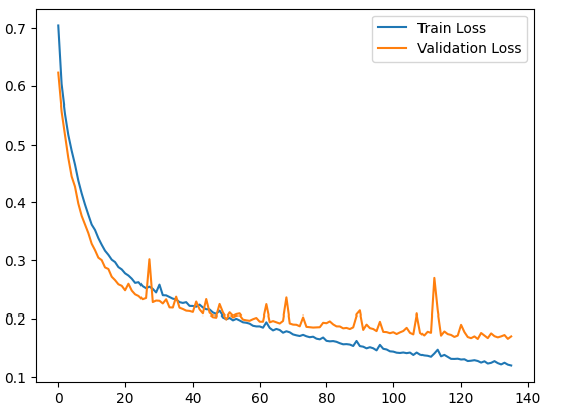
\includegraphics[width=0.75\textwidth]{learningcurve1}
    \caption{Kod çalıştığındaki train ve validation loss değerleri}
    \label{fig:my_pic}
\end{figure}


\subsection{(10 Puan)} \textbf{SEED=öğrenci numaranız set ettikten sonra altıncı haftada ödev olarak verdiğim gibi earlystopping'deki en iyi modeli kullanarak, Prensesi İyileştir test setinden accuracy, F1, precision ve recall değerlerini hesaplayan kodu yazın ve sonucu da aşağı yapıştırın. \%80'den fazla başarı bekliyorum test setinden. Daha düşükse başarı oranınız, nerede hata yaptığınızı bulmaya çalışın. \%90'dan fazla başarı almak mümkün (ben denedim).}

\begin{python}
model.eval()
with torch.no_grad():
    y_pred = model(test_x).squeeze().numpy()
    y_pred_rounded = [round(pred) for pred in y_pred]
    acc = accuracy_score(test_y, y_pred_rounded)
    f1 = f1_score(test_y, y_pred_rounded)
    precision = precision_score(test_y, y_pred_rounded)
    recall = recall_score(test_y, y_pred_rounded)

print(f'Accuracy: {acc:.4f}')
print(f'F1 Score: {f1:.4f}')
print(f'Precision: {precision:.4f}')
print(f'Recall: {recall:.4f}')
\end{python}

Accuracy: 0.9391

F1 Score: 0.9372

Precision: 0.9723

Recall: 0.9046

\subsection{(5 Puan)} \textbf{Tüm kodların CPU'da çalışması ne kadar sürüyor hesaplayın. Sonra to device yöntemini kullanarak modeli ve verileri GPU'ya atıp kodu bir de böyle çalıştırın ve ne kadar sürdüğünü hesaplayın. Süreleri aşağıdaki tabloya koyun. GPU için Google Colab ya da Kaggle'ı kullanabilirsiniz, iki ortam da her hafta saatlerce GPU hakkı veriyor.}

\begin{table}[ht!]
    \centering
    \caption{Buraya bir açıklama yazın}
    \begin{tabular}{c|c}
        Ortam & Süre (saniye) \\\hline
        CPU & 93 \\
        GPU & 91\\
    \end{tabular}
    \label{tab:my_table}
\end{table}

\subsection{(3 Puan)} \textbf{Modelin eğitim setine overfit etmesi için elinizden geldiği kadar kodu gereken şekilde değiştirin, validasyon loss'unun açıkça yükselmeye başladığı, training ve validation loss'ları içeren figürü aşağı koyun ve overfit için yaptığınız değişiklikleri aşağı yazın. Overfit, tam bir çanak gibi olmalı ve yükselmeli. Ona göre parametrelerle oynayın.}

Cevaplar buraya

% Figür aşağı
\begin{comment}
\begin{figure}[ht!]
    \centering
    \includegraphics[width=0.75\textwidth]{mypicturehere.png}
    \caption{Buraya açıklama yazın}
    \label{fig:my_pic}
\end{figure}
\end{comment}

\subsection{(2 Puan)} \textbf{Beşinci soruya ait tüm kodların ve cevapların olduğu jupyter notebook'un Github linkini aşağıdaki url'e koyun.}

\href{https://github.com/ilkay-bicici/yapaysiniraglariornekler/blob/83e7c9b6202ea32adf1ece1eeadc6e4ed62ac409/curetheprincess.ipynb}{Multi Layer Perceptron GitHub Linki}

\section{(Toplam 10 Puan)} \textbf{Bir önceki sorudaki Prensesi İyileştir problemindeki yapay sinir ağınıza seçtiğiniz herhangi iki farklı regülarizasyon yöntemi ekleyin ve aşağıdaki soruları cevaplayın.} 

\subsection{(2 puan)} \textbf{Kodlarda regülarizasyon eklediğiniz kısımları aşağı koyun:} 

\begin{python}
import torch.nn as nn
#Dropout Regularization
class MLP(nn.Module):
    def __init__(self):
        super(MLP, self).__init__()
        self.hidden1 = nn.Linear(train_x.shape[1], 100)
        self.relu1 = nn.ReLU()
        self.dropout1 = nn.Dropout(p=0.3)
        self.hidden2 = nn.Linear(100, 50)
        self.relu2 = nn.ReLU()
        self.dropout2 = nn.Dropout(p=0.3)
        self.output = nn.Linear(50, 1)
        self.sigmoid = nn.Sigmoid()

    def forward(self, x):
        x = self.hidden1(x)
        x = self.relu1(x)
        x = self.dropout1(x)
        x = self.hidden2(x)
        x = self.relu2(x)
        x = self.dropout2(x)
        x = self.output(x)
        x = self.sigmoid(x)
        return x
\end{python}

\begin{python}
l1_lambda = 0.000001
# Egitim asamasi - L1 Regularization
    model.train()
    train_loss = 0.0
    train_count = 0.0
    for x_batch, y_batch in train_loader:
        optimizer.zero_grad()
        y_pred = model(x_batch).squeeze()
        l1_norm = sum(p.abs().sum() for p in model.parameters())
        loss = criterion(y_pred, y_batch) + l1_lambda * l1_norm
        loss.backward()
        optimizer.step()
        train_count += 1.0
        train_loss += loss.item()
\end{python}

\subsection{(2 puan)} \textbf{Test setinden yeni accuracy, F1, precision ve recall değerlerini hesaplayıp aşağı koyun:}

Accuracy: 0.9469

F1 Score: 0.9456

Precision: 0.9753

Recall: 0.9175

\subsection{(5 puan)} \textbf{Regülarizasyon yöntemi seçimlerinizin sebeplerini ve sonuçlara etkisini yorumlayın:}

Modelin overfitting yapmasının önüne geçmek amacıyla ve ikisini bir arada kullanınca nasıl bir sonuç vereceğini merak ettiğimden L1 ve Dropout regülarizasyon yöntemlerini kodun ilgili kısımlarına ekledim.

Sonuçlara bakılırsa, regülarizasyonların eklenmesi modelin doğruluk (Accuracy), F1 skoru (F1 Score), Precision ve duyarlılık (Recall) değerlerini arttırmıştır. Bu da modelin genelleme yeteneğinin arttığını göstermektedir.

\subsection{(1 puan)} \textbf{Sonucun github linkini  aşağıya koyun:}

\href{https://github.com/ilkay-bicici/yapaysiniraglariornekler/blob/83e7c9b6202ea32adf1ece1eeadc6e4ed62ac409/curetheprincesswithregularization.ipynb}{Multi Layer Perceptron With Regularization GitHub Linki}

\end{document}